\documentclass[11pt]{article}
\usepackage{amsmath,amsfonts,amsthm,amssymb,mathtools, color}
\usepackage{tikz}

\begin{document}

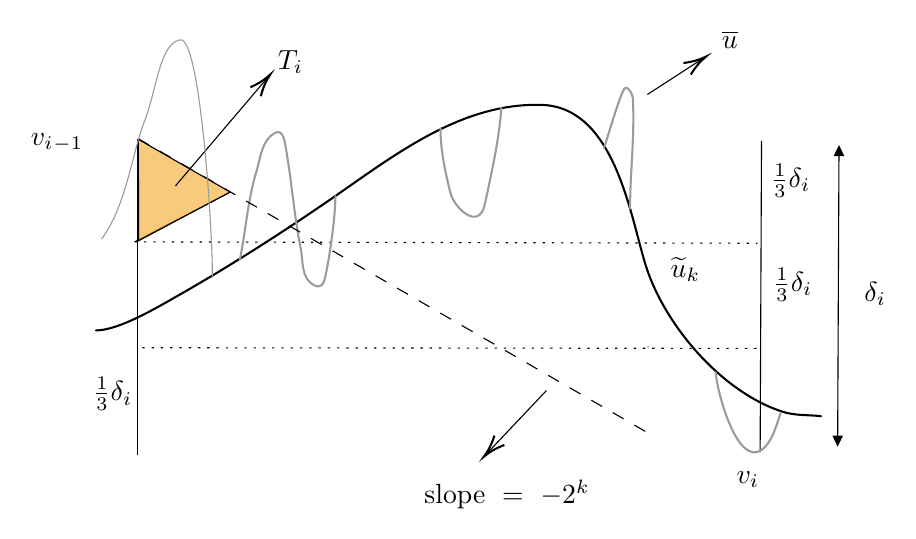
\begin{tikzpicture}[x=0.75pt,y=0.75pt,yscale=-1,xscale=1]

\draw    (160.33,221.67) -- (160.33,69.67) ;
\draw    (461,70.33) -- (460.33,220.33) ;
\draw  [dash pattern={on 0.84pt off 2.51pt}]  (159,119) -- (459,119.67) ;
\draw  [dash pattern={on 0.84pt off 2.51pt}]  (162.67,170) -- (459,170.33) ;
\draw    (498.32,75.33) -- (497.68,214.67) ;
\draw [shift={(497.67,217.67)}, rotate = 270.26] [fill={rgb, 255:red, 0; green, 0; blue, 0 }  ][line width=0.08]  [draw opacity=0] (5.36,-2.57) -- (0,0) -- (5.36,2.57) -- cycle    ;
\draw [shift={(498.33,72.33)}, rotate = 90.26] [fill={rgb, 255:red, 0; green, 0; blue, 0 }  ][line width=0.08]  [draw opacity=0] (5.36,-2.57) -- (0,0) -- (5.36,2.57) -- cycle    ;
\draw  [line width=0.75] [line join = round][line cap = round] (140.33,161.67) .. controls (151.45,161.67) and (170.74,150.07) .. (179.67,145) .. controls (204.34,130.99) and (228.27,115.68) .. (251.67,99.67) .. controls (282.71,78.43) and (315.28,51.87) .. (355,53) .. controls (389.93,54) and (397.54,105.16) .. (405,129.67) .. controls (413.88,158.86) and (442.03,191.8) .. (471.67,201) .. controls (477.43,202.79) and (483.74,202.26) .. (489.67,203) ;
\draw  [color={rgb, 255:red, 155; green, 155; blue, 155 }  ,draw opacity=1 ][line width=0.75] [line join = round][line cap = round] (406.33,169.67) .. controls (406.33,169.67) and (406.33,169.67) .. (406.33,169.67) ;
\draw  [color={rgb, 255:red, 155; green, 155; blue, 155 }  ,draw opacity=1 ][line width=0.75] [line join = round][line cap = round] (209.67,127.67) .. controls (212.45,113.74) and (213.54,98.43) .. (217.67,85) .. controls (219.53,78.94) and (220.31,69.2) .. (227,66.33) .. controls (230.66,64.76) and (231.37,71.35) .. (231.67,73) .. controls (234.73,90.04) and (235.7,105.84) .. (239,122.33) .. controls (240.11,127.87) and (239.14,136.41) .. (245,139.67) .. controls (248.98,141.88) and (250.11,139.32) .. (251,135) .. controls (253.08,124.88) and (255.67,107.27) .. (255.67,97) ;
\draw  [color={rgb, 255:red, 155; green, 155; blue, 155 }  ,draw opacity=1 ][line width=0.75] [line join = round][line cap = round] (306.33,64.33) .. controls (306.33,74.67) and (308.54,84.96) .. (311,95) .. controls (312.97,103.06) and (324.94,113.74) .. (327.67,101) .. controls (330.88,86) and (334.56,69.77) .. (335.67,54.33) ;
\draw  [color={rgb, 255:red, 155; green, 155; blue, 155 }  ,draw opacity=1 ][line width=0.75] [line join = round][line cap = round] (385,73.67) .. controls (385.73,72.93) and (392.24,49.26) .. (395,45) .. controls (396.11,43.28) and (398.89,47.62) .. (399,49.67) .. controls (399.97,68.42) and (397.67,85.02) .. (397.67,103) ;
\draw  [color={rgb, 255:red, 155; green, 155; blue, 155 }  ,draw opacity=1 ][line width=0.75] [line join = round][line cap = round] (438.97,181.83) .. controls (439.29,190.58) and (449.71,229.7) .. (462.13,218.38) .. controls (466.32,214.56) and (468.4,206.73) .. (470.12,201.64) ;
\draw    (159,119) -- (205,95) ;
\draw  [dash pattern={on 4.5pt off 4.5pt}]  (160.72,69.31) -- (409.67,213) ;
\draw  [fill={rgb, 255:red, 245; green, 166; blue, 35 }  ,fill opacity=0.6 ] (205,95) -- (160.9,118.46) -- (160.74,69.59) -- cycle ;
\draw    (178.67,92) -- (223.04,39.86) ;
\draw [shift={(224.33,38.33)}, rotate = 130.4] [color={rgb, 255:red, 0; green, 0; blue, 0 }  ][line width=0.75]    (10.93,-3.29) .. controls (6.95,-1.4) and (3.31,-0.3) .. (0,0) .. controls (3.31,0.3) and (6.95,1.4) .. (10.93,3.29)   ;
\draw    (357.33,190.67) -- (328.57,221.08) ;
\draw [shift={(327.2,222.53)}, rotate = 313.4] [color={rgb, 255:red, 0; green, 0; blue, 0 }  ][line width=0.75]    (10.93,-3.29) .. controls (6.95,-1.4) and (3.31,-0.3) .. (0,0) .. controls (3.31,0.3) and (6.95,1.4) .. (10.93,3.29)   ;
\draw    (406,48) -- (432.65,30.75) ;
\draw [shift={(434.33,29.67)}, rotate = 147.09] [color={rgb, 255:red, 0; green, 0; blue, 0 }  ][line width=0.75]    (10.93,-3.29) .. controls (6.95,-1.4) and (3.31,-0.3) .. (0,0) .. controls (3.31,0.3) and (6.95,1.4) .. (10.93,3.29)   ;
\draw [color={rgb, 255:red, 155; green, 155; blue, 155 }  ,draw opacity=1 ]   (143,117.67) .. controls (155,101.67) and (157.67,76.33) .. (163.67,61) .. controls (169.67,45.67) and (171,23.12) .. (181,21.67) .. controls (191,20.22) and (197,122.33) .. (196.33,135.67) ;

% Text Node
\draw (509.33,137.07) node [anchor=north west][inner sep=0.75pt]    {$\delta _{i}$};
% Text Node
\draw (464.33,80.4) node [anchor=north west][inner sep=0.75pt]
{$\frac{1}{3} \delta _{i}$ };
% Text Node
\draw (137.67,183.07) node [anchor=north west][inner sep=0.75pt]
 {$\frac{1}{3} \delta _{i}$ ~};
% Text Node
\draw (465.33,130.4) node [anchor=north west][inner sep=0.75pt]
 {$\frac{1}{3} \delta _{i}$};
% Text Node
\draw (416,125.4) node [anchor=north west][inner sep=0.75pt]
 {$\widetilde{u}_{k}$};
% Text Node
\draw (107.7,65.4) node [anchor=north west][inner sep=0.75pt]
{$v_{i}{}_{-1}$};
% Text Node
\draw (447.7,228.4) node [anchor=north west][inner sep=0.75pt]
{$v_{i}$};
% Text Node
\draw (226.67,25.73) node [anchor=north west][inner sep=0.75pt]
 {$T_{i}$};
% Text Node
\draw (297.33,232.4) node [anchor=north west][inner sep=0.75pt]
 {$\mathrm{slope} \ = \  -2^{k}$};
% Text Node
\draw (440.67,16.07) node [anchor=north west][inner sep=0.75pt]
  {$\overline{u}$};


\end{tikzpicture}

\end{document}